\documentclass[11pt]{article}
\usepackage{latexsym}
\usepackage{amsmath}
\usepackage{amssymb}
\usepackage{amsthm}
\usepackage{epsfig}
\usepackage{psfig}
\usepackage{url}
\usepackage{algorithm}
\usepackage{algorithmic}
% \usepackage[pdftex]{graphicx}
\usepackage{subfig}
\usepackage{color}
\usepackage{xcolor}
\usepackage{listings}

\usepackage{caption}
\DeclareCaptionFont{white}{\color{white}}
\DeclareCaptionFormat{listing}{\colorbox{gray}{\parbox{\textwidth}{#1#2#3}}}
\captionsetup[lstlisting]{format=listing,labelfont=white,textfont=white}




% 1-inch margins, from fullpage.sty by H.Partl, Version 2, Dec. 15, 1988.
\topmargin 0pt \advance \topmargin by -\headheight \advance \topmargin by
-\headsep \textheight 8.9in \oddsidemargin 0pt \evensidemargin \oddsidemargin
\marginparwidth 0.5in \textwidth 6.5in

\parindent 0in \parskip 1.5ex
% \renewcommand{\baselinestretch}{1.25}

\begin{document}

\title{Truthfulness Verification System}

\author{
Tathagata Dasgupta, ABM Musa\\
Email: \{tdasgu2, amusa2\}@uic.edu }

\date{}
\maketitle


\section{Introduction}
Web has became most prevalent source of information now a days. However, many
information on the web is untruthful. Also because of the widespread reach of
web, sometimes web is used to propagate untruthful facts for social and political
reasons. Hence with the increasingly use of web as information source,
verification of information truthfulness became an important facet to consider.

The popular search engines extract information from web based on keywords and
metadata without considering the truthfulness of the facts. Also, there have been
not much research in this area. To our best knowledge, the most recent work on this area is T-verifier  \cite{tverifier}, which uses results from search engines
to verify truthfulness of statements. T-verifier performs very well on the
test-dataset. However, T-verifier has some problems with the overall approach to
verify the truthfulness of statements and there is room for improvement. In this
work, we will extend the T-verifier system so that it's weaknesses can be
resolved to get a more robust truthfulness verification system.


\section{Current System}
Current system for truthfulness verification is called T-verifier
\cite{tverifier}, which uses two phase methods for truthfulness verification of
statements. Each of these two phases rely heavily on search results returned by
popular search engines. T-verifier takes the doubtful statements (DS) as input
from the user along with the doubtful unit (DU). Phrase after removing DU from DS
is called topic unit (TU).

At the first phase, T-verifier generates alternative statements by supplying
$TU$ to search engine and collecting the relevant alternate $DU$-s. However,
from basic web search may result in lot of alternate DUs that are not semantically or
logically relevant to the original DS. Hence, T-verifier uses combination of
seven features to rank alternate DUs. These features primarily exploit the facts
that relevant alternative units frequently co-occur, people often mention both
misconception and truthful conception together, data-type matching, and
sense-closeness. T-verifier chooses top 5 alternative statements based on top 5
alternate DUs obtained in this phase.

At the second phase, top 5 alternative statements from phase 1 is supplied to the
search engine again. Then the returned searched result is ranked by multiple
rankers such as Alternative Unit Ranker, Hits ranker, Text-feature Ranker, Domain
Authority Ranker etc. Then all those ranks are merged to form an overall ranking
among the alternate statements and top statement in this final merged ranking is
considered as truthful statement.

% We are currently working to get the T-verifier code running on our systems,
% with inputs from Xian Li. So the descriptions below lacks some required details
% and makes some assumptions.   As of now T-Verifier produces 5 alternative
% statements once it is provided with a doubtful statement (DS), a doubtful unit
% (DU), data type of the unit etc in the first phase. Though these sentences
% produced are quite accurate, the facility to pinpoint the correct alternative
% does exist yet. The project goal, may be formulated as:  "Extract information
% from Wikipedia and ontologies ( such as Yago, DBpedia and Freebase) which helps
% to verify truthfulness of statements. Describe the extraction algorithm and how
% the information can be utilized to assist statement truthfulness verification."

\section{Problems with Current System}
Although results from the tested dataset achieves good performance (90\%
accuracy), failing of T-verifier for some statements shows that it has some
inherent problems and there is room for improvement.

First, T-verifier assumes that truthful statements will be more propagated in the
web compared to the untruthful statement. However, this may be not true in
general because of intended and planned propaganda for establishing some
untruthful statements. This kind of propagandas are even becoming more common now
a days due to widespread reach of Internet. T-verifier also showed that "Hillary
Clinton is the President of United States" has more hits than "Hillary Clinton is
the Secretary of State". Although T-verifier was able to find the correct
statement in this case using multiple ranks together, in general the untruthful
statement can be prevalent in the web compared to truthful statements.

Second, T-verifier do not use the reputation of the information source.
T-verifier uses only search results returned by the search engine irrespective of
the origin and believability of the information origin. Hence there is room for
improvement here to give more weight to the information obtained from trustworthy
sources such as Wikipedia.


\section {Propsed System}


\begin{figure}
  \centering
  \subfloat[System
  overview]{\label{fig:System}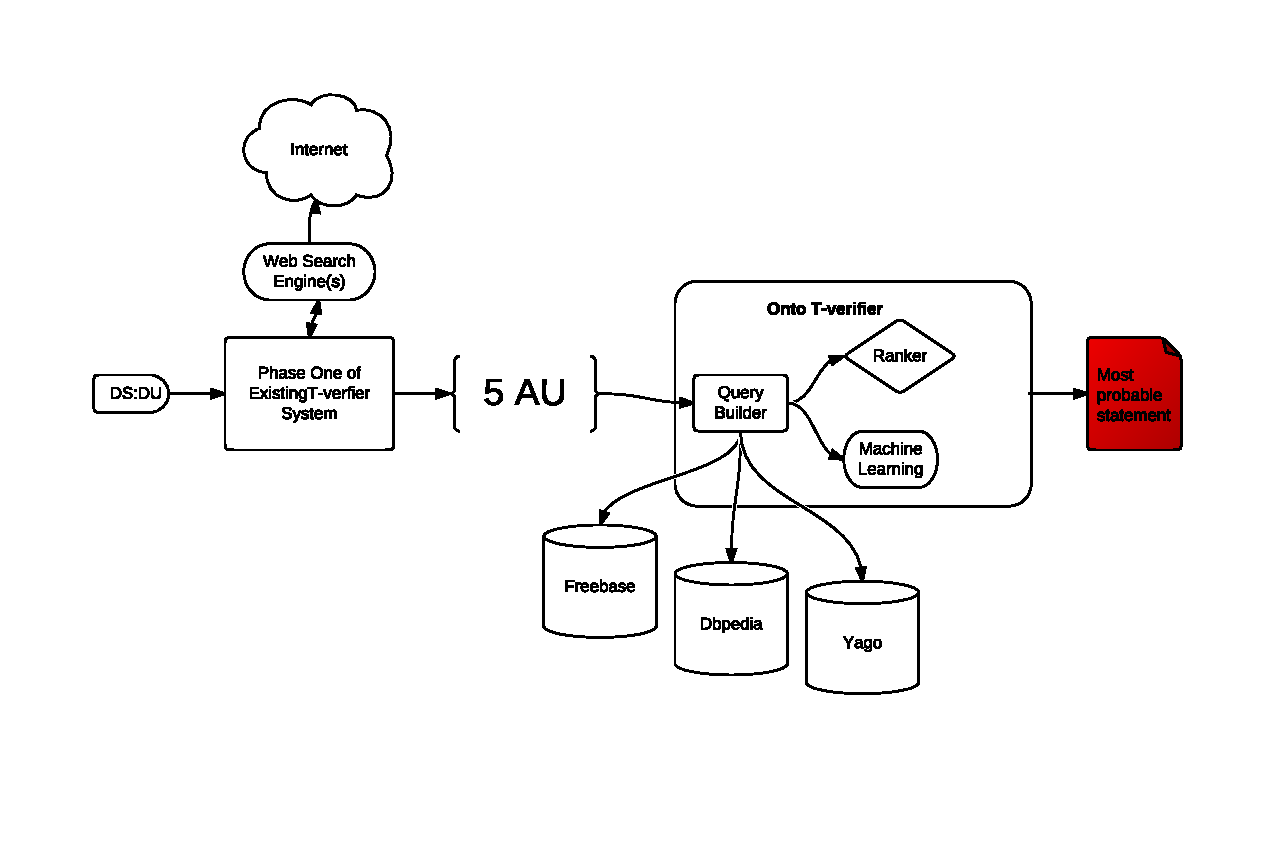
\includegraphics[width=0.85\textwidth]{system.pdf}}
  \caption{System overview}
  \label{fig:system}
\end{figure}


\subsection{Description of extraction algorithm}

For disambiguation among the alternative statements, Wikipedia is generally used
as an authoritative source. However, the contents of Wikipedia is not available
in the form that is consumable in a programmatic format. To address such
difficulties a number of projects Yago, DBpedia, Freebase have organized the
massive amount of data in a searchable fashion e.g DBpedia uses SPARQL endpoint,
Freebase uses MQL api. Open source implementation of Python wrappers exist for
both the interfaces exist and appear to be mature enough for our needs.

\subsubsection{Freebase} 
Freebase has information about approximately 20 million Topics, each one having a
unique Id, which can help distinguish multiple entities which have similar names,
such as Henry Ford the industrialist vs Henry Ford the footballer. Most of the
topics are associated with one or more types\cite{freebasetype} (such as
people, places, books, films, etc) and may have additional properties like "date of birth" for a person
or latitude and longitude for a location. Freebase not only contains data from
the Wikipedia but also other sources; users can submit data to the Freebase
datastore and expand it in richness. We tinkered with the api\cite{freebaseapi}
and it appeared to be the most viable starting point for the project.

\subparagraph{Motivational Example}

\begin{lstlisting}[label=some-code,caption=Minimal code to Freebase]

import freebase
import pprint

query = [{
  "a:starring": [{
    "actor": "Meg Ryan"                                                       
  }],
  "b:starring": [{                                                            
    "actor": "Tom Hanks"
  }],
  "type": "/film/film",
  "*": [],
}]  
    
pp = pprint.PrettyPrinter(indent=4)
result = freebase.mqlread(query)
    
print "Movie names & their various forms"
    
    
for i in result:                                                              
        pp.pprint(i["key"])                                                   
                
\end{lstlisting}
\begin{lstlisting}[label=output,caption=Cleaned Output]

Movie names & their various forms
[   '158982',
    'You$0027ve_Got_Mail',
    '18171032',

     ...
    'E-m$0040il_f$00FCr_Dich',
    'youve-got-mail']
[   '176489',
    'Joe_Versus_the_Volcano',
    'Joe_Vs$002E_The_Volcano',
    'Brain_Cloud',
     ...
    '2327353',
    'joe-versus-the-volcano']
[   '226198',
    'Sleepless_in_Seattle',
    'Sleepless_In_Seattle',
     ....
    '169146',
    '106482',
    'Insonnia_d$0027amore',
    '62812',
    'Schlaflos_in_Seattle',
    'sleepless-in-seattle'\]

\end{lstlisting}

The above results show how the three movies starring Tom Hanks and Meg Ryan.
When we query Google with Tom Hanks and Meg Ryan, the top result is a page from
Answers.com where a user has asked which are the movies where the two actors
appear together, and the answer lists these three movies namely - ``Joe versus
the Volcano'', `` Sleepless in Seatle'' and ``You\'ve got Mail''. A quick lookup
of the Wikipedia and IMDB pages also confirm the same. 

\subsubsection{Dbpedia}
DBpedia is a similar project to Freebase, but it focuses mainly on the content
available from Wikipedia. It scores in being precisely importing the data from
the info boxes in Wikipedia pages, but at this stage it does not seem to be
offering anything additional over Freebase \cite{freebasedbpedia}. We are yet to
explore its programmatic interface \cite{dbpediaapi}.


\subsubsection{Yago}
YAGO is a semantic knowledge base with over 900,000 entities (like persons,
organizations, cities, etc.) and uses Wikipedia and Wordnet as its main source of
information. We are yet to explore the programmatic interfaces it provides and
how we can use it for the project.




\subsection{Truthfulness verification }
\subsubsection {Building queries from the data supplied by the user}

We take the content words from the topic unit($TU$), along with each of the
alternative units($AU$), and plugin the datatype($t$) to form a number of
queries.
\begin{align*}
q_{i} = \{{TU, AU_{i}, t_{AU_{i}}} \} \qquad \mbox {where $i = 1 \cdots n$} \\
\end{align*}
where $n$ is the number of alternative units generated by the first phase of
the existing system. By quering the various ontologies described above we will
get results which might have the following cases:

\begin{align*}
   freebase(q_{i}) &= \phi \\
    = r_{i}
\end{align*}

From what we have explored till now, by quering Freebase we can get the
various property, value pairs associated with an entity which is the $TU$ in
our case. In case the result is $\phi$, it suggests that we do not have
information for this particulat combination $TU$ and $AU_{i}$. Due to the richness of the information in Freebase we can assume with a considerable degree of confidence
that this combination is untrue. This is one way verification, but in case of
non-null results, how do we filter and rank the results with the available set
of information is something we can not formulate at this stage with out further
exploration.

\subsubsection{Finding Sense using Wordnet}
To classify a statement as true or false we need to get the semantic of sense of the words of the sentences. For example consider the following sentence. 

\emph{"Tom Hanks was the lead actress in the movie sleepless in Seattle"}

Now our query results from ontologies will give us the fact that Tom hanks is a male actor. Now using wordnet we will be able to find that actress means female actor. So by simple inference our system will be able to classify the above example as untruthful.

\subsubsection{Use of Co-reference Program}
Totha: please write up two lines here



\subsubsection{Application of Machine learning algorithms}
Though usage of machine learning algorithm seems to be a good approach at
this point. Consider the following example.

\emph{"Tom Hanks was the lead actress in the movie sleepless in Seattle"}

Now If the algorithm can learn that Tom hanks is a male and so he can't be an actress then our system should be able to classify the above statement as false. 

However, we will need to explore more to be sure that we can apply machine learning algorithms successfully. Supervised classifiers might not be beneficial for us due to the limited dataset for training and the potentially unlimited variety of inputs to classify. However, if we can use Graph Based Partially Supervised Learning\cite{conf/acl/CelikyilmazTH09} or Spreading Activation \cite{Cohen1987255} on the information extracted from the rich ontologies is something we plan to explore.


\section{Conclusion}
It this paper, we described current system for truthfulness verification of statements found in the web called T-Verifier and described the possible improvements to the current system. We will primarily use authentic information sources such as Wikipedia and Ontologies extracted from Wikipedia such as FreeBase, DBPedia, and YOGA to found the truthfulness of doubtful statements.  


\bibliographystyle{plain}
\bibliography{ref}

\end{document}

